\documentclass{article}[18pt]
\usepackage{../../../../format}
\lhead{Networks and Systems - Networks}
\newcommand\filledcirc{{\color{black}\bullet}\mathllap{\circ}}

\begin{document}
\begin{center}
\underline{\huge Network Layer}
\end{center}
\section{Routing Algorithms}
Routing is the process of discovering network paths
\begin{itemize}
	\item Decide what to optimize (e.g., fairness vs efficiency)
	\item Model the network as a graph of nodes and links
	\item Update routes for changes in topology (e.g. failures)
\end{itemize}
\section{Optimality Principle}
Identify the optimal path from source to destination
\begin{defin}[Sink tree]
Optimal routes from all sources to a given destination
\end{defin}
Distance metric: the number of hops, or time delay
\section{Shortest Path Algorithm}
Dijkstra's algorithm computes a sink tree on the graph
\begin{itemize}
	\item Each node is labelled with its distance from the source node to the best known path
	\item Initially no paths are known
	\item Each link is assigned a non-negative weight/distance
	\item Shortest path is the one with the lowest total weight
\end{itemize}
Algorithm
\begin{itemize}
	\item Start with sink, set distance at other nodes to infinity
	\item Labels tentative ($\circ$) or permanent ($\filledcirc$), initially all tentative
	\item Pick the lowest distance non-permanent node, make it permanent
	\item Repeat from this node, until all nodes are permanent
\end{itemize}
\section{Distance vector routing}
There are two dynamic routing algorithms
\subsection{Distance vector}
\begin{itemize}
	\item Each node maintains a table (vector of best known destination)
	\item Tables are updated by exchanging information between nodes
	\item Tables have 2 entries: \textbf{outgoing line} and \textbf{estimated distance} (\# hops or propagation delay)
\end{itemize}
Algorithm:
\begin{itemize}
	\item Each node knows distance of links to its neighbours
	\item Each node advertises a vector of the lowest known distances to all neighbours
	\item Each node uses received vectors to update its own
	\item Repeat periodically
\end{itemize}
\begin{center}
	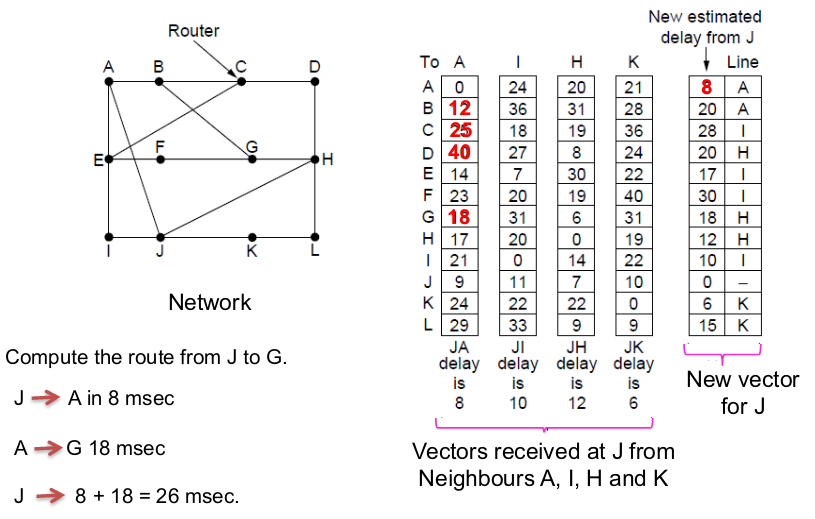
\includegraphics[scale=0.7]{distance_vector_routing}
\end{center}
\subsubsection{The Count-to-Infinity Problem}
Failures can cause DV to "count to infinity" while seeking a path to an unreachable node
\begin{center}
	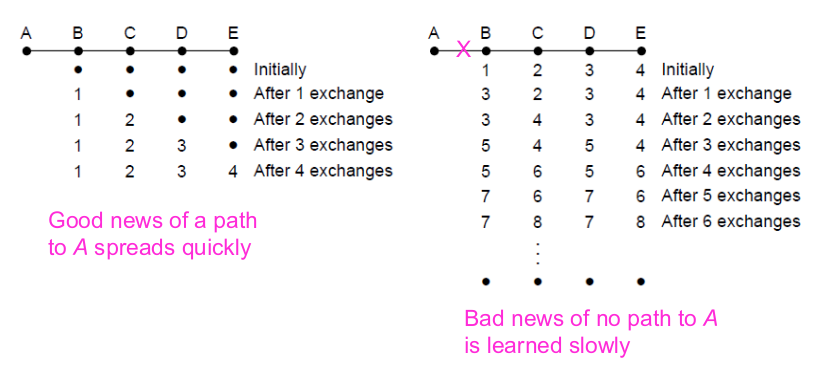
\includegraphics[scale=0.7]{infinity}
\end{center}
\subsection{Link State Routing}
Link state is an alternative to distance vector algorithm. There are 5 steps:
\begin{enumerate}
	\item Learn the network address of the neighbouring routers by sending HELLO packet, record name
	\item Set the distance to each neighbour
	\item Construct a packet telling all other routers what it has just learned
	\item Send the packet to neighbours and receive packet from all other routers
	\item Compute the shortest path by using Dijkstra's algorithm
\end{enumerate}
\begin{defin}[LSP (Link State Packet)]
A list of the node's neighbours and weights of links to reach them
\end{defin}
\begin{center}
	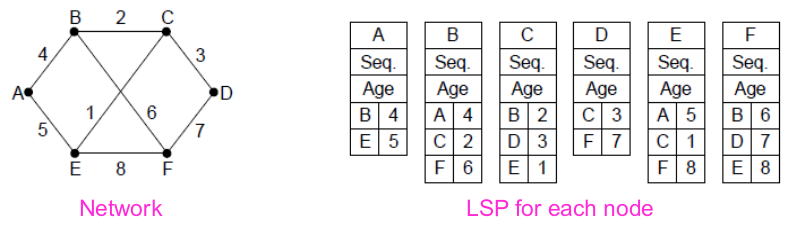
\includegraphics[scale=0.7]{LSP}
\end{center}
\section{Hierarchical Routing}
Hierarchical routing reduces the work of route computation but may result in slightly longer paths than flat routing
\begin{center}
	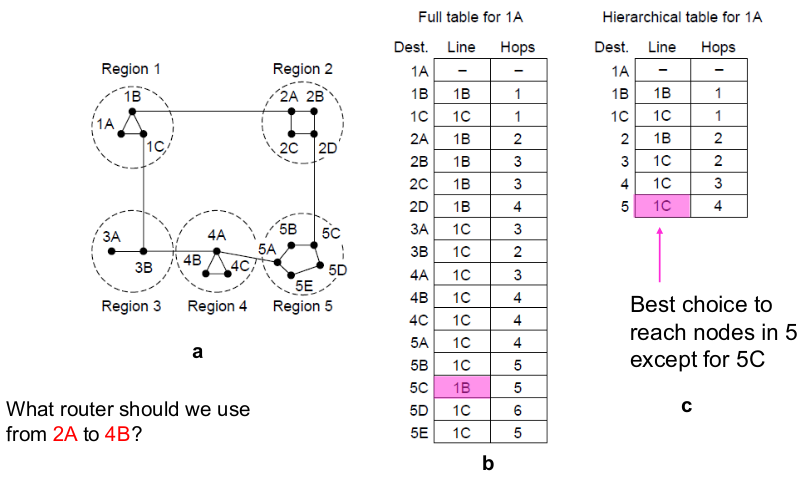
\includegraphics[scale=0.7]{Hierarchical}
\end{center}
Useful in the internet, each region would be geographical, makes routing much faster to compute.
\section{Flooding}
\begin{itemize}
	\item A simple method to send a packet to all network nodes
	\item Each node floods a new packet received on an incoming link by sending it out of the other links
	\item Nodes need to keep track of flooded packets to stop the flood
\end{itemize}
\section{Broadcasting}
Broadcast sends a packet to all nodes:
\begin{itemize}
	\item RPF (Reverse Path Forwarding): Arrived packets are checked to see if they arrived from a preferred link, which is the link that is normally used for sending packets towards the source of the broadcast
	\item 1st hop: I sends packets to F, H J and N. Packets arrive on the same link that is used to send to I
	\item 2nd hop: 8 packets are generated, two by each router. 5 of them arrive on the preferred link
\end{itemize}
\begin{center}
	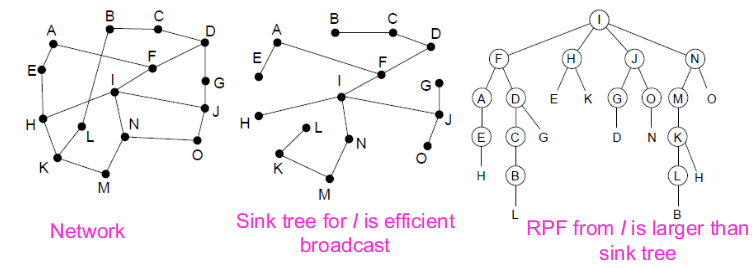
\includegraphics[scale=0.7]{Broadcast}
\end{center}


\end{document}